\subsubsection{Hall-interrupt funktion}
\label{Hall-funktion}

Hall-interrupt funktionen er delt op i tre dele: Preround, Mapping round og Run time. I alle delene benytter vi Hastigheds funktionen, som sætter hastigheden, såfremt den får den ønskede hastighed, samt den aktuelle hastighed som input.

\begin{figure}
\begin{center}
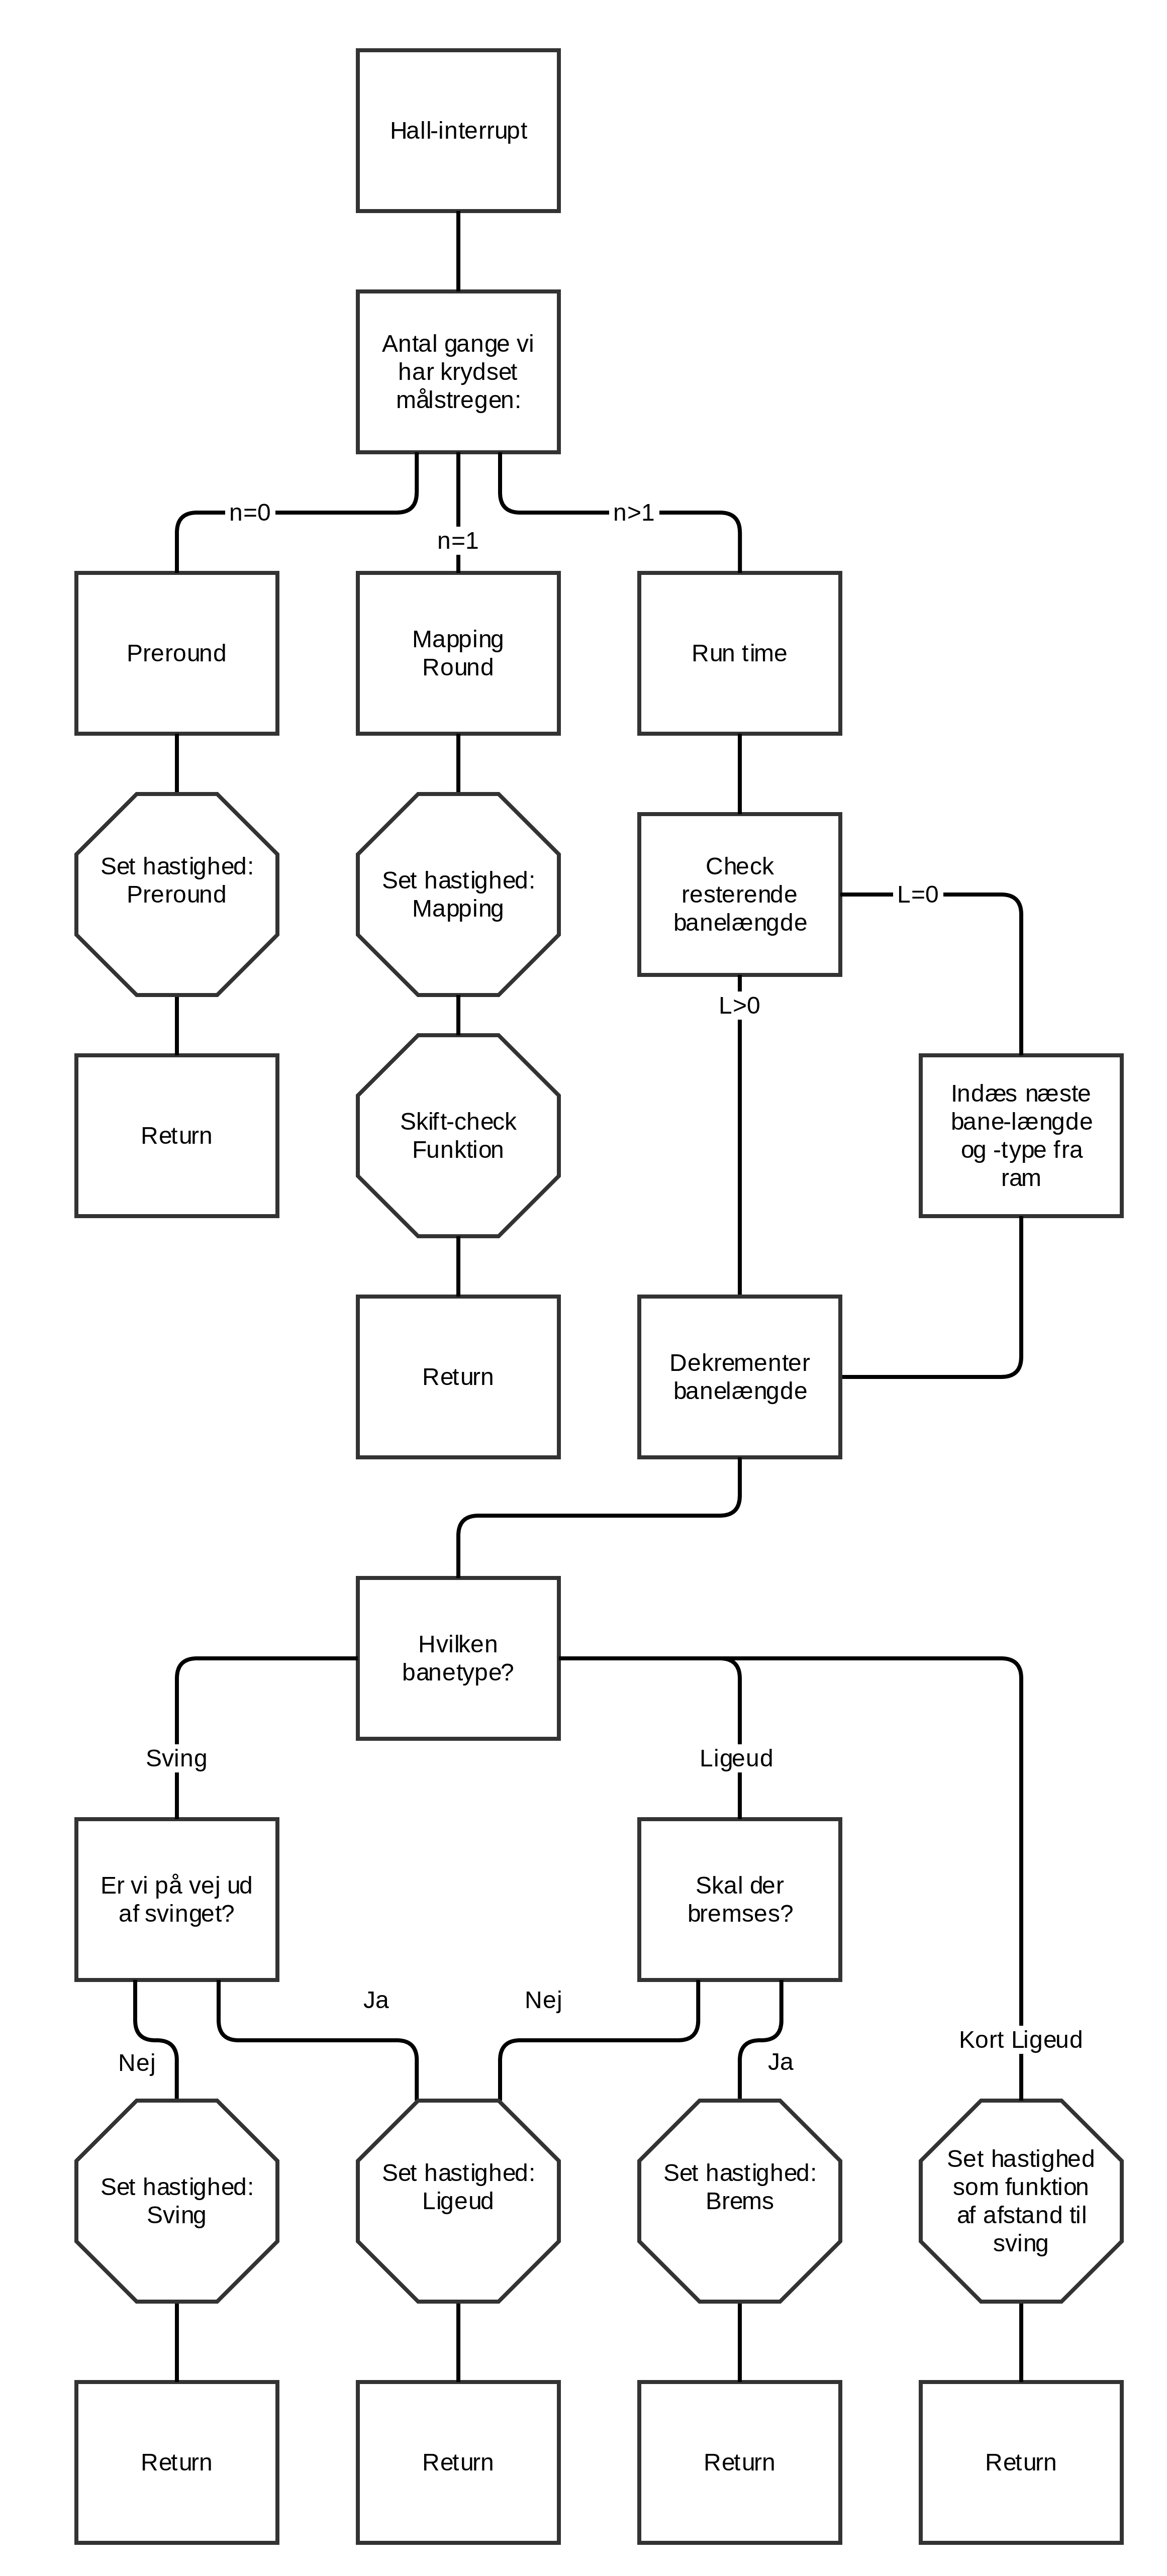
\includegraphics[scale=0.1]{Billeder/hall_interrupt.png}
\end{center}
\caption{Flowchart der beskriver Hall-interrupt funktionen. De ottekantede kasser er funktioner der er beskrevet i andre flowcharts.}
\label{fig:Hall Flowchart}
\end{figure}

\subsubsection{Hall-interrupt ved Preround}

I Preround skal bilen bare holde en stabil hastighed, så her aktiverer vi blot vores Hastigheds Call-funktion.

\subsubsection{Hall-interrupt ved Mapping round}

Når Hall sensoren laver et interrupt, ved microcontrolleren at der er kørt en tolvtedel af en hjulomdrejning. Dette betyder at vi meget præcist, i forhold til blot at bruge hele, halve, eller kvarte hjulomdrejninger, kan mappe længden af forskellige bane elementer op. Vi bestemmer, ved brug af gyroen, den vinkelhastighed vi har i øjeblikket, og sammenligner denne med de satte værdier for de forskellige banetyper. Hvis resultatet er det samme, som den gemte banetype inkrementerer vi blot banelængden. Ellers undersøger vi om skiftet er mellem et lille og et stort sving. Da vinkelhastigheden er større for et lille sving, vil bilen altid tro, at der er tale om et stort sving på vej ind og ud af et sving. Derfor gemmer vi ikke vejlængden, hvis der er tale om et skift mellem et stort og lille sving, men ændrer blot typen til at være et stort sving. Hvis skiftet er mellem et stort sving og et lige banestykke, gemmer vi det forrige banestykke som længde og type i rammene, og sætter længden på det nye stykke til at være 1. Se figur \ref{fig:Skift Flowchart} for visuel repræsentation.

\subsubsection{Hall-interrupt ved Run time}

I Main round benytter vi vores map til at bestemme, hvilken hastighed bilen skal køre med. Ved først at bestemme om mappet siger at bilen er på et lige banestykke, et lille sving eller et stort sving, kan vi se hvilken hastighed, bilen burde køre med. Vi ser så, om vi er på vej ind eller ud af et sving. Hvis vi er på vej ind i et sving bremses der . Hvis vi er på vej ud af et sving sættes ``hastigheden'' til at være det samme som på et lige banestykke.
\\
Når vi kører ind i et lige stykke, checker vi om der er tale om et stykke, hvor der er tid til at gasse nok op, til at der skal bremses ned. Hvis der ikke er, sætter vi en hastighed, der afhænger af afstanden til det næste sving.
\\
 Derefter sendes der en tilsvarende ønsket hastighed til Hastigheds Call funktionen.